\chapter{Tasks and Methods}
\label{TaskAndMethods}
The scope of this chapter is to use the Concepts from Chapter 5 and the understanding of the current design process to generate the tasks, in which user involvement is considered helpful in the design and development of the TonePrint community. The tasks focus on how to acquire the necessary information from the users to design different features or how to evaluate already made decisions. The objective of some of the tasks may also be to simply get a better understanding of the users themselves. A general insight into the users' perspective will help optimize the general utilization of usability and UX at TC Electronic, even though the direct objective of the specific study doesn't have a direct relation to usability or UX. After providing a description of the tasks and the need for user involvement for these individual instances, proposals for applicable methods for uncovering usability or UX in their respective contexts will then be presented. One of the tasks will then be selected to be carried out during the last phase of this project.

% \section{Tasks for developing the Community}
% \label{TasksForDevelopingTheCommunity}
% Write some description of how the tasks is determined and can be categorized. 

%Define the task - What is the goal?
%How can this be investigated? - Which methods can be applied for it?
%What is the realistic time aspect for applying these methods? How long do they take? / How are they best applied for the design process at TC Electronic? (SCRUM)
%%What equipment and how many subjects are required?

\section{Task 1: Designing the information architecture}
\label{Task1}
When designing the TonePrint community, it's important to consider the structure of the information, better known as information architecture. The purpose of this is to ensure that the design accommodates the users' mental model in terms of being a closer match to the conceptual model of the system. This would ease the use of the system, as the system would act accordingly to the users' expectations. As explained in Chapter 4, TC Electronic haven't acquired information about their users understanding of the TonePrint application before, which makes this task even more important. two ways of approaching this will be addressed. \\

\noindent
One approach could be to involve the users early on while designing the system by letting them take part in shaping the concept and flow of the community. This is also referred to as a \textit{participatory design procedure} \footnote{Participatory design methods in telemedicine research}. During this, the users are provided a chance of influencing the design of a future product for example by conducting workshops with them as participants. In the case of the TonePrint community, these workshops could for example be set up with multiple steps focusing on different aspects of the information architecture. This could include a brainstorming session for creating conceptual ideas for the community, a card sorting task where these ideas are grouped, and a session for creating prototypes from these groups. Another approach also focusing on the information architecture could be to test the current thoughts and ideas of how the application should be structured through prototype testing. Low fidelity (Lo-fi) prototypes comes to mind in this context. These are used to test the functionality of an application even though a functional prototype isn't available. Instead prototypes are constructed from easy accessible materials without spending much time on the aesthetic appearance. Usually, subjects are asked to complete tasks on prototypes sketched on paper. For the TonePrint community, lo-fi prototyping can as such be employed to indicate how the functionalities and features shall be shaped, through user tests with the information structure in focus. This makes lo-fi prototypes very usefull to employ, however, they require a rough idea of how the system should work and how the information is going to presented before conducting the actual test. When brainstorming possible methods for testing with lo-fi prototypes, \textit{the cognitive walkthrough} comes to mind as a suitable suggestion. Through this method, the subjects are given a number of tasks to complete on the prototype, where each task has a well defined action sequence necessary to follow step-by-step in order complete the task correctly. The subjects' results are then analyzed through general principles of cognitive psychology in order to locate potential pitfalls in the design.\\

\noindent
For either of the tasks above, some preparation is necessary. firstly in the case of constructing lo-fi prototypes, the necessary materials are needed to create a fitting representation. For a participatory design workshop, there are some materials required depending on the sessions in the workshop, but in general, generic elements such as post-it notes for the brainstorming session are needed. The subjects required for participating, whatever the approach, need to account for the possible end-users of the TonePrint community, which means musician, sound engineers, novice and expert TonePrint users, etc. Hopefully, several different groups can take part in this, as a clear representation of each group's understanding of what the engineers conceive as useful tools is desired. The process of acquiring the subjects can be eased with the help of TC Electronic themselves though their existing community on Facebook among others. For the cognitive walkthrough the subjects don't necessarily require the same level of background knowledge, as it can be conducted with novices and experts alike, depending on the chosen approach. As such, the members of the development teams at TC Electronic could also be used as subjects for the test.\\

\begin{figure}[H]
	\centering
	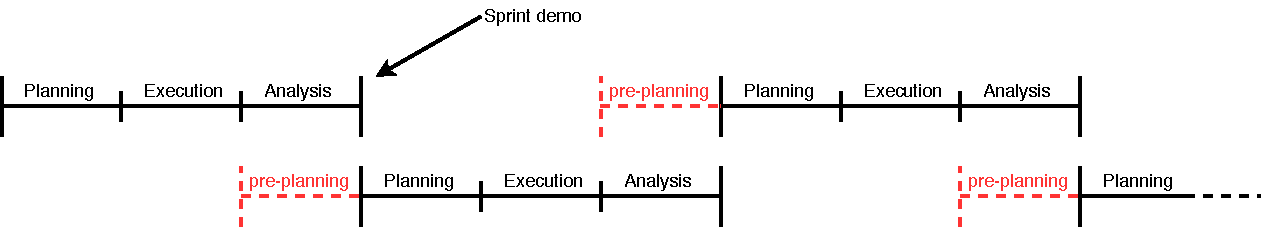
\includegraphics[width=\textwidth]{SprintFitExample.pdf}
	\caption{An illustration of how to fit minor user studies to the SCRUM framework. Each sprint period is split into weekly intervals with the final week also functioning as a pre-planning phase for the next sprint.}
	\label{fig:SprintFitExample}
\end{figure}
\noindent


% starThet of the design process  scope is to design a system which accommodates the users mental model in terms of being close to the developers conceptual model.\\
%(Opgaven er at designe det så udviklernes konceptuelle model matcher brugernes mental model)\\
%As seen in \autoref{ThemanticAnalysis} is..........
%2 bud til informationsstrukturen:
%- konkret tests
%Vi kan lave forslag til, hvordan det skal se ud og så lave en test, der undersøger, hvad der fungerer, og hvad der ikke fungerer - Eksempelvis med en cognitive walktrhough
%- Participary design phase:
%Vi har et konkret mål, vi skal opnå med de her elementer, hvordan vil brugerne sætte det sammen? - eksempelvis med papirstykker, de skal placere, så det giver mening.
%Er der fordele i at trække nogle paralleler fra andre systemer i forhold til designet af communitiet? - Skal vi bruge 100p rigtige brugere, eller kan vi sætte noget op med genereiske brugere?

\section{Task 2: Tags}
\label{Task2}
%Define the task - What is the goal?
%How can this be investigated? - Which methods can be applied for it?
%What is the realistic time aspect for applying these methods? How long do they take? / How are they best applied for the design process at TC Electronic? (SCRUM)
%What equipment and how many subjects are required?

%Define the task - What is the goal?
A new feature in the TonePrint Community is the 'tag' feature which is described in point 2 in \autoref{tab:ListOfCommunityFeatures}. Furthermore is it conceptualized in the conceptual model \autoref{fig:CommunityConceptualModel} and the use case \autoref{fig:CommunityConceptualUseCase}, and is based on the interview  with the development team \autoref{InterviewConclusion}. From the interview it's clear that the fist task related to tags is to investigate how tags can be made feasible and distinguishable for users. To accommodate this, some decision should be taken regarding to which extend the users should be limited in their choice of tag. If every user is allowed to assign tags without any constrains, could would be difficult for other users to have clear expectations regarding towards what a TonePrint sounds like, because of subjective opinions could affect the understanding of tags. To accommodate this could the TonePrint community generate tag suggestions based on the parameter settings , from which the TonePrint creator than would choose from. The tags which the user would pick from would in other words be "Effect describing categories" This leads to a task defining which parameters based tags users would be able to use to describe their TonePrint, and to what extend its possible to distinguish between tags.

\noindent
%How can this be investigated? - Which methods can be applied for it?
For accommodating this task a sensory analysis like study could be conducted with at group a representative subjects. The participants would be given a tasks of rating different auditory stimuli consisting of TonePrints on scales representing the effect describing categories. Depending on how the ratings are clustered in groups it would indicate the users ability to distinguish the TonePrints on the basis of the effect describing categories. These ratings would indicate to what extend the effects can be distinguished, which than would indicate naturals level of tags, which than could be given names \footnote{Skal det nævnes at der efter den sensoriske analyse kunne laves en card sort analyse for at se om der er enighed om hvordan de her 'Tags' høre sammen og evntuelt et forsøg hvor de fremstillede tas skal gives til nogle stimuli}. Before conducting this experiment it's necessary to create the effect describing categories. This could fore instance be done by having a word elicitation session where attributes which may describe a TonePrint stimuli is determined. These attributes would than either be used directly or as inspiration fore creating, effect describing categories.\\

\noindent
%What is the realistic time aspect for applying these methods? How long do they take? / How are they best applied for the design process at TC Electronic? (SCRUM)
The time expected for accommodating this task by using the explained method would probably reach more than one sprint cycle. This is partially doe to the need of at least two separate sessions (Word elicitation and sensory analysis), from which the latter should be conducted for several effect types and with several different effect describing categories. It would be possible to fit one experiment at a time accordingly with a sprint. 

%The task regarding tags is to generate evaluate the users understanding of the depth of tags. Firstly it has to be determined to what extend the tags would be limited by the parameters settings. If there is no limitations the users would be able to chose among every setting, which could compromise how the effect of the tags, when used for searching desired tags. The first phase of this task would be to figure out how TC can analyze a the parameters settings of a TonePrint, and present it as effect describing categories. Than it would be possible to conduct a sesory analysis like study, where different auditory stimuli would be rated on the effect describing categorize. These ratings would indicate to what extend the effects can be distinguished, which than would indicate naturals level of tags, which than could be given names.\\
%The Time schedule of this method would be to extensive at this point of the project and will there for not be included (Det skal laves, dog ikke n'dvændigt på nuværende tidspunkt da vi ikke skal lave dette forsøg, grundet mangel på tid)
%Which types of tags should be used to mark TonePrints (Pedal type?, genre?, Something subjective)\\
%hvordan giver man tags, og hvordan søger man efter det (Både grafisk og konceptuelt)\\
%Hvordan forsår brugerne tags og hvordan vil de bruge det?
%Tags:
%Analyse af deres eksisterende database om TonePrints - Er der nogle naturlige grupperinger, der dukker op, som kan bruges som tags?
%Rop er ikke fan
%Hvis man vil gå ind og lave word elicitation, skal man forholde sig til nogle ting, der allerede er predefineret - fx effekttype i forhold til pedaler
%Overordnede  kategorier, der er systemdefineret
%herefter kommer der de mere subjektive indelinger - fx et eksempel på en systemdefineret tag kunne være Flanger, herefter kan en subjektiv inddeling beslutte, om hvor mange typer flanger, man skal have.

\section{Task 3: Self-promoting functionalities}
\label{Task3}
It's necessary to have a functional community before looking at how much users will like to promote them self and how they will like to do it. Here it might be a good idea to look at other systems based on user created content, which is shared with others. Users with experience of creating User TonePrints would be included in a explorative evaluation of these other systems, evaluating the amount and type of self promotion. This evaluation could lead to qualitative data which should indicate the users expected attitude towards how the self promotion factors should be designed.\\
(At sætte en test op hvor man gennemgår et andet systems måde at gøre det på, vil muligvis ikke være optimalt i fohold til den tid det vil tage, kontra det man får ud af det. Måske bør det sættes op sådan at man laver en prototype baseret på en analyse af hvordan andre gør, som så kan bruges i test scenarier. Det vil dog alt sammen kun afspegle forventet brug, da brugernes actuelle brug vil kunne ændre sig i den rigtige TonePrint Community)

%Skal brugerne have mulighed for at promovere ders TonePrints og dem selv? (Hvis ja, hvordan - ala facebook eller soundcloud?)
%Self-promoting functionalities:
%Rop synes, det vil være vigtigere blot at kunne lægge et TonePrint ud, så andre brugere kan forstå, hvor det er ud fra navn eller lidt information
%Det vil være dumt at prøve at opfinde hjulet igen - Rops holdning er helt klart at kigge på lignende sociale medier etc. og anvende analogier derfra.
%Man er nødt til at have et aktivt community før man kan tage diskussionen om elvpromoveringen

\section{Task 4: Appearance and GUI of the App}
\label{Task4}
%Define the task - What is the goal?
From the name of this task, it seems as the scope of it is the same as that of task 1, this is however not the case. Task 1 aims to approach the design of the information structure from scratch, either by conducting user tests on specific design proposals or by approaching it as a \textit{participatory design phase} with excessive user involvement. The scope of this task moves beyond just the information structure, as it can concern any aspects of the functionality and aesthetics of the GUI. As students of engineering psychology, such a task could easily resemble that of a typical semester project. The logical approach would be to conduct user tests on existing products in order to propose eventual re-designs, and in the case of the TonePrint concept, it could for example be the application or a design proposal for a community platform.\\

\noindent
%How can this be investigated? - Which methods can be applied for it?
At this point, TC Electronic don't conduct user tests to the extend of UX-designers, but it is a field, they are interested in exploring further. Design proposals are currently decided upon by the graphical designers in the firm, and a way of involving users could be to either confirm or reject these proposals through an A/B test scenario. In this, different design proposals are scientifically tested, comparing them to each other by measuring the effects of different assignments on the users' behavior. the two variables A and B usually consists of a currently used version and another version modified in correlation with what the focus of the test is. The differences between the designs should be small and concern specific elements, as the method is particularly valuable when there isn't a vast number of variables. As an example, the method could be applied to the TonePrint app by testing a part of the interface that has been modified in an alternate version where the rest of the interface remains unchanged. If the scope of the test is concerning an evaluation of the entire system, either as a stand-alone evaluation or in comparison with a re-designed version, methods are also applicable for this approach, even though a comparison of two versions with multiple variables is considered risky. The UX-designer needs to have a clear idea of what is wanted from the test, and if the scope of interest for example is an evaluation of the system's overall usability, the \textit{System Usability Scale (SUS)} comes to mind as an applicable method. This is a quick and dirty, reliable tool that consists of 10 questions, intended to uncover the system's usability through a somewhat complex scoring system. The resulting score can nevertheless be evaluated by itself or in comparison with the SUS score from a modified system.\\

\noindent
%What is the realistic time aspect for applying these methods? How long do they take? / How are they best applied for the design process at TC Electronic? (SCRUM)
In the well planned scenario, conducting such a user test should be easy, as it isn't considered time-consuming if all the variables are understood and decided upon. Depending on the state of the design process, it can either be conducted as a low-fidelity or a high-fidelity test. For the A/B test, it would be preferable to conduct the test at an early stage with a lo-fi approach, as the specifications for the design elements still might be up for discussion. In order to best manage the variables in the test, TC should consider focusing on individual elements and test them one at a time. This would furthermore be a good way of applying it to the Scrum framework, as a test shouldn't take more than 3 weeks to plan, execute, and analyze. In a hypothetical scenario, the graphical designers and programmers at TC could spend a sprint on designing and implementing a functionality, which then would be the focus of a user test in the following sprint. A UX-designer could then spend the first week planning, how they best uncover the important aspect from the user, spend the second week executing this, and during the analysis of the final week, they could already begin planning the scope of the user test for the following sprint. The developers would simultaneously be working on implementing the next feature, and this would make the argument for the UX-designers to participate in the daily scrum meetings to the same extend as the developers. The UX-designer would get a look into what they are working on and as such be able to think ahead for the next sprint.\\

\noindent
%What equipment and how many subjects are required?
Conducting such a test requires the involvement of the developers, as they implement the functionality that is of interest in the test. a UX-designer should discuss with them, what they want to uncover from the test and then apply his knowledge of how to uncover this. In the case of simply being interested in usability, the UX-designer would then gather a number of unbiased subjects and have them perform a task with the new functionality in focus. The following evaluation could then simply be the subjects filling out a system usability scale. In the case of an A/B test, the materials required would be an alternate version to the current, either constructed as a paper prototype or through wire-framing software. Groups of users would then be assigned to interact with each of the different designs, uncovering their experience for each of these instances through different measurements and questioning. 


\section{Task 5: Defining the user groups}
\label{Task5}
The purpose of this task is to ease the process of designing and developing the TonePrint community by getting a better understanding of who the users are. By having a clear understanding of the users, it's easier to get the design right, faster, and it will require fewer individual user studies. If the developers can make decisions from simply asking themselves "how would the users react and perform to this feature?" much time and resources can be spared on recruiting subjects and conducting user tests \parencite{WEB:PersonasIDF}. From this description, the ideal approach seems to be constructing \textit{personas} of the typical TonePrint users. In general, personas serve as archetypes of the users who you can turn to when asking the previously mentioned question of "how would person X react and perform to this feature?" instead of designing these features by the preferences of the design team. For this description, the approach developed by \textcite{WEB:PersonaKilde} is emphasised as a preferable way of creating personas. She proposes 10 steps for this, going from collecting data on the users to finding patterns and developing the actual personas, before defining the need of the persona and disseminating this knowledge to the members of the development team. The 10 steps are obviously more comprehensive than just presented here and elaborated on in more details by \citeauthor{WEB:PersonaKilde} herself \parencite[][9]{WEB:PersonaKilde}. Her recipe is however not the only way of creating personas, as this general topic has existed since the late 1990s. in literature on personas there are today four other approaches to engage with. \citeauthor{WEB:PersonaKilde} elaborates on these herself, but they can also found from a simple web search \parencite{WEB:PersonasIDF}. They are as followed:
%
\begin{enumerate}
    \item \textbf{Goal-directed Personas}
    \item \textbf{Role-based Personas}
    \item \textbf{Engaging Personas}
    \item \textbf{Fictional Personas}
\end{enumerate}
%
\noindent
The goal-directed personas intends to uncover what the typical user wants to do with a system in question by examining their workflow while trying to complete an objective with the system. By understanding the goals of the users, it's easier to fit the necessary requirements within the system to make these objectives easy to perform for the users. The role-based personas should also be considered goal-directed but focuses more on behaviour by examining the user's role in a wider perspective. For example by understanding where the product will be used and what the purpose of the user's role is, it can help the design team make better design decisions for the product. The engaging persona method is a way of getting more engaged with the users, as the method employs both a goal and role-directed approach. Typically, a 3D rendering of the user is created from this method, which will make the developers more likely to consider them during the design process, their emotions, and their psychological background. Finally, the fictional personas don't emerge from user research but instead from the experience of the UX design team. Based on past interactions with the user base, the team makes assumptions of what users look like. This can be debated as a flawed approach, but it does allow for considerations of the user's needs at an early stage \parencite[][11]{WEB:PersonaKilde}.\\

\noindent
Having these personas seems as an ideal guideline for making design decisions for the system in question, however, constructing these personas isn't something done easily over a 3-week sprint period. The process includes multiple steps of first finding the users, collecting data on the their patterns within different user groups and then describing and validating these findings. as such, extensive interview sessions and observational studies of the users interacting with the system in question is required. For this project, this task is therefore considered too extensive for a 2-week period, but for TC's future work on the TonePrint community, a design approach with personas is considered ideal.

As previously mentioned, the personas method requires a lot of data collection, preferably from interviews and observational studies, and while clear-cut explanations of how to create personas exist, this paper also proposes an alternative approach. For all the tasks listed in this section, different proposals have been made on how to engage them with different types of user involvement. besides providing a helping hand in the decision making for the design of the TonePrint community, Each of these proposals also provide individual minor descriptions of the users in the context of the individual user studies. Another approach to defining the user groups could therefore be to gather descriptions of the users through these individual user studies and create the personas on the basis of them. The benefit of such an approach is that the developers could kill two birds with one stone while conducting user studies on different features for the TonePrint community. they would simply gather the needed information from multiple smaller user studies.
